\documentclass[11pt,a4paper]{article}

% Math
\usepackage{amsmath}
\usepackage{amssymb}
\usepackage{amsfonts}

% Graphics and figures
\usepackage{graphicx}

% Tables
\usepackage{booktabs}
\usepackage{array}

% Code listings
\usepackage{listings}
\usepackage{xcolor}

% Hyperlinks
\usepackage[hidelinks]{hyperref}

% Better captions
\usepackage{caption}

% Float placement
\usepackage{float}

% Page margins
\usepackage[margin=1in]{geometry}

\usepackage{cleveref}
\usepackage{siunitx}
\usepackage{mathtools}

\usepackage{amsmath}
\usepackage{amssymb}
\usepackage{amsfonts}
\numberwithin{equation}{section}
\usepackage{tikz}
\usetikzlibrary{
    arrows.meta,
    positioning,
    shapes.geometric,
    calc
}

\begin{document}
\begin{center}
\begin{Large}
    \textbf{Implementation of State Estimation for Bipedal Robot}
\end{Large}
\\
Van Thanh Nguyen\\
Winter - 2026
\end{center}

\section{StateEstimateBase Class}

The \texttt{StateEstimateBase} class is an abstract base class used for state estimation in the legged robot framework. It provides common functionality for handling:

\begin{itemize}
    \item Joint encoder measurements
    \item IMU measurements
    \item Contact state information
    \item Robot state storage
    \item Odometry publishing
\end{itemize}

The actual estimation algorithm is implemented in derived classes through the pure virtual function \texttt{update()}.

\subsection{Class Purpose}

The class maintains the robot state vector

\begin{equation}
x =
\begin{bmatrix}
q \\
\dot{q}
\end{bmatrix},
\end{equation}

where \(q\) denotes the generalized coordinates and \(\dot{q}\) denotes the generalized velocities.

The state is stored in

\begin{lstlisting}[language=C++]
vector_t rbdState_;
\end{lstlisting}

which is initialized as

\begin{lstlisting}[language=C++]
rbdState_(vector_t::Zero(
    2 * info_.generalizedCoordinatesNum))
\end{lstlisting}

so that

\begin{equation}
\texttt{rbdState} =
\begin{bmatrix}
q \\
\dot{q}
\end{bmatrix}.
\end{equation}

\subsection{Constructor}

The constructor is defined as

\begin{lstlisting}[language=C++]
StateEstimateBase(
    rclcpp::Node::SharedPtr node,
    PinocchioInterface pinocchioInterface,
    CentroidalModelInfo info,
    const PinocchioEndEffectorKinematics&
        eeKinematics);
\end{lstlisting}

Its responsibilities are:

\begin{enumerate}
    \item Store the ROS node handle.
    \item Store the Pinocchio interface.
    \item Store robot model information.
    \item Clone the end-effector kinematics object.
    \item Allocate the state vector.
    \item Create odometry and pose publishers.
\end{enumerate}

\subsection{State Vector Layout}

Let

\begin{equation}
N = \texttt{info\_.generalizedCoordinatesNum}.
\end{equation}

The state vector layout is

\begin{table}[h]
\centering
\begin{tabular}{cl}
\hline
Indices & Description \\
\hline
0--2 & Base orientation (ZYX Euler angles) \\
3--5 & Base position \\
6-- & Joint positions \\
\hline
$N+0$ -- $N+2$ & Base angular velocity \\
$N+3$ -- $N+5$ & Base linear velocity \\
$N+6$ -- & Joint velocities \\
\hline
\end{tabular}
\caption{Layout of \texttt{rbdState}.}
\end{table}

\subsection{Joint State Update}

The function

\begin{lstlisting}[language=C++]
updateJointStates(
    const vector_t& jointPos,
    const vector_t& jointVel);
\end{lstlisting}

stores the encoder measurements into the state vector:

\begin{align}
\texttt{rbdState}(6 : 6+n_j-1)
    &= \texttt{jointPos}, \\
\texttt{rbdState}(N+6 : N+6+n_j-1)
    &= \texttt{jointVel},
\end{align}

where \(n_j\) is the number of actuated joints.

\subsection{Contact State Update}

The function

\begin{lstlisting}[language=C++]
updateContact(contactFlag);
\end{lstlisting}

stores the current foot contact configuration.

This information is later used by state estimation algorithms such as:

\begin{itemize}
    \item Linear Kalman Filters
    \item Contact-aided localization
    \item Base velocity estimation
\end{itemize}

\subsection{Locomotion Mode}

The function

\begin{lstlisting}[language=C++]
size_t getMode();
\end{lstlisting}

converts the contact pattern into a locomotion mode identifier:

\begin{equation}
\texttt{mode}
=
\texttt{stanceLeg2ModeNumber(contactFlag)}.
\end{equation}

Typical modes include:

\begin{itemize}
    \item Left stance
    \item Right stance
    \item Double support
    \item Flight phase
\end{itemize}

\subsection{IMU Update}

The function

\begin{lstlisting}[language=C++]
updateImu(...)
\end{lstlisting}

processes IMU measurements.

Its inputs include:

\begin{itemize}
    \item Orientation quaternion
    \item Angular velocity
    \item Linear acceleration
    \item Covariance matrices
\end{itemize}

The procedure is:

\begin{enumerate}
    \item Store raw IMU measurements.
    \item Convert quaternion to ZYX Euler angles.
    \item Remove orientation offset.
    \item Convert local angular velocity into the representation required by OCS2.
    \item Update the angular state.
\end{enumerate}

\subsubsection{Quaternion to Euler Conversion}

The orientation is represented as

\begin{equation}
q =
\begin{bmatrix}
w & x & y & z
\end{bmatrix}^{T}.
\end{equation}

The helper function

\begin{lstlisting}[language=C++]
quatToZyx(q)
\end{lstlisting}

returns

\begin{equation}
\boldsymbol{\theta}
=
\begin{bmatrix}
\psi \\
\theta \\
\phi
\end{bmatrix},
\end{equation}

where

\begin{itemize}
    \item \(\psi\): yaw
    \item \(\theta\): pitch
    \item \(\phi\): roll
\end{itemize}

\subsection{Angular State Update}

The function

\begin{lstlisting}[language=C++]
updateAngular(
    const vector3_t& zyx,
    const vector_t& angularVel);
\end{lstlisting}

stores

\begin{align}
\texttt{rbdState}(0:2)
    &= \texttt{zyx},\\
\texttt{rbdState}(N:N+2)
    &= \texttt{angularVel}.
\end{align}

Therefore, the state contains both orientation and angular velocity.

\subsection{Linear State Update}

The function

\begin{lstlisting}[language=C++]
updateLinear(
    const vector_t& pos,
    const vector_t& linearVel);
\end{lstlisting}

stores

\begin{align}
\texttt{rbdState}(3:5)
    &= \texttt{pos},\\
\texttt{rbdState}(N+3:N+5)
    &= \texttt{linearVel}.
\end{align}

These correspond to the floating-base position and velocity.

\subsection{State Estimation Interface}

The function

\begin{lstlisting}[language=C++]
virtual vector_t update(
    const rclcpp::Time& time,
    const rclcpp::Duration& period) = 0;
\end{lstlisting}

is pure virtual and must be implemented by derived classes.

A typical implementation performs:

\begin{enumerate}
    \item Read IMU measurements.
    \item Read joint encoder measurements.
    \item Read contact information.
    \item Estimate base position and velocity.
    \item Update the state vector.
    \item Publish odometry.
\end{enumerate}

\subsection{Odometry Publishing}

The function

\begin{lstlisting}[language=C++]
publishMsgs(const nav_msgs::msg::Odometry& odom);
\end{lstlisting}

publishes

\begin{itemize}
    \item \texttt{/odom}
    \item \texttt{/pose}
\end{itemize}

at a fixed rate of approximately

\begin{equation}
f = 200\ \text{Hz}.
\end{equation}

Realtime ROS publishers are used to ensure thread-safe communication.

\subsection{Class Architecture}

The overall data flow is illustrated in Figure~\ref{fig:state_estimation_flow}.

\begin{figure}[htbp]
\centering

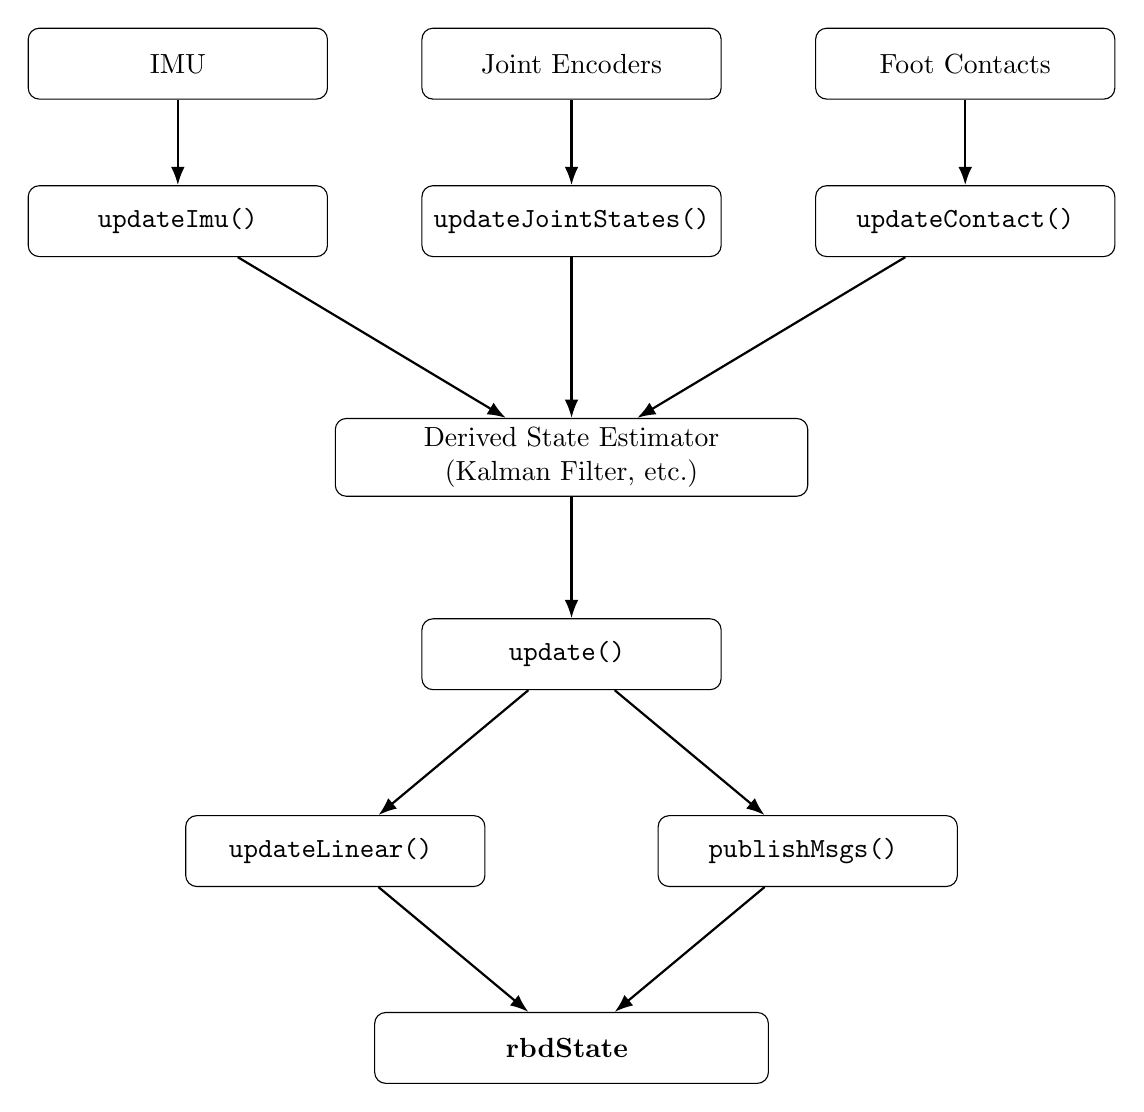
\begin{tikzpicture}[
    >=Latex,
    block/.style={
        rectangle,
        draw,
        rounded corners,
        align=center,
        minimum width=3.8cm,
        minimum height=0.9cm
    },
    line/.style={
        -Latex,
        thick
    }
]

%--------------------------------------------------
% Row 1 : Sensors
%--------------------------------------------------

\node[block] (imu) at (0,0) {IMU};

\node[block] (joint) at (5,0)
    {Joint Encoders};

\node[block] (contact) at (10,0)
    {Foot Contacts};

%--------------------------------------------------
% Row 2 : Update functions
%--------------------------------------------------

\node[block] (uimu) at (0,-2)
    {\texttt{updateImu()}};

\node[block] (ujoint) at (5,-2)
    {\texttt{updateJointStates()}};

\node[block] (ucontact) at (10,-2)
    {\texttt{updateContact()}};

%--------------------------------------------------
% Row 3 : Estimator
%--------------------------------------------------

\node[block,
      minimum width=6cm]
      (estimator)
      at (5,-5)
{
Derived State Estimator\\
(Kalman Filter, etc.)
};

%--------------------------------------------------
% Row 4 : update()
%--------------------------------------------------

\node[block] (update)
    at (5,-7.5)
{
\texttt{update()}
};

%--------------------------------------------------
% Row 5
%--------------------------------------------------

\node[block] (linear)
    at (2,-10)
{
\texttt{updateLinear()}
};

\node[block] (publish)
    at (8,-10)
{
\texttt{publishMsgs()}
};

%--------------------------------------------------
% Row 6
%--------------------------------------------------

\node[block,
      minimum width=5cm]
      (state)
      at (5,-12.5)
{
$\mathbf{rbdState}$
};

%--------------------------------------------------
% Connections
%--------------------------------------------------

\draw[line] (imu) -- (uimu);
\draw[line] (joint) -- (ujoint);
\draw[line] (contact) -- (ucontact);

\draw[line] (uimu) -- (estimator);
\draw[line] (ujoint) -- (estimator);
\draw[line] (ucontact) -- (estimator);

\draw[line] (estimator) -- (update);

\draw[line] (update) -- (linear);
\draw[line] (update) -- (publish);

\draw[line] (linear) -- (state);
\draw[line] (publish) -- (state);

\end{tikzpicture}

\caption{Architecture of the \texttt{StateEstimateBase} framework.}
\label{fig:state_estimation_architecture}

\end{figure}

In summary, \texttt{StateEstimateBase} provides a common interface for sensor handling, state storage, and ROS communication, while derived classes implement the actual state estimation algorithm.
\newpage
\section{Linear Kalman Filter State Estimation}

The \texttt{KalmanFilterEstimate} class implements a discrete-time linear Kalman filter for estimating the floating-base position and velocity of a legged robot. The filter fuses information from:

\begin{itemize}
\item IMU linear acceleration,
\item Joint encoder measurements,
\item Foot kinematics,
\item Foot contact states.
\end{itemize}

\subsection{State Vector}

Assume the robot has $(n_c)$ contact points. The state vector is defined as

\begin{equation}
\mathbf{x} =\begin{bmatrix}
\mathbf{p}_b \
\mathbf{v}_b \
\mathbf{p}_{f_1} \
\hdots \
\mathbf{p}_{f_{n_c}}
\end{bmatrix}
\in \mathbb{R}^{6+3n_c},
\end{equation}

where

\begin{itemize}
\item ($\mathbf{p}_b \in \mathbb{R}^{3})$ is the base cartesian position,
\item ($\mathbf{v}_b \in \mathbb{R}^{3})$ is the base cartesian/linear velocity,
\item ($\mathbf{p}_{f_i} \in \mathbb{R}^{3})$ is the world-frame position of foot (i).
\end{itemize}

Therefore,

\begin{equation}
n_x = 6 + 3n_c .
\end{equation}

\subsection{System Dynamics}

The state propagation model is

\begin{equation}
\mathbf{x}_{k+1} = \mathbf{A}\mathbf{x}_k
+
\mathbf{B}\mathbf{a}_k
+
\mathbf{w}_{k},
\end{equation}

where

\begin{equation}
\mathbf{a}_k
= \mathbf{R}_{WB}\mathbf{a}_{imu}
+
\mathbf{g}
\end{equation}

is the IMU acceleration expressed in the world frame.

The state transition matrix is

\begin{equation}
\mathbf{A}=
\begin{bmatrix}
\mathbf{I}_3 & \Delta t \mathbf{I}_3 & \mathbf{0} \\
\mathbf{0} & \mathbf{I}_3 & \mathbf{0} \\
\mathbf{0} & \mathbf{0} & \mathbf{I}_{3n_c}
\end{bmatrix},
\end{equation}

which corresponds to

\begin{align}
\mathbf{p}_{b,k+1}
&=
\mathbf{p}_{b,k}
+
\Delta t \mathbf{v}_{b,k},
\\
\mathbf{v}_{b,k+1}
&=
\mathbf{v}_{b,k}.
\end{align}

The control-input matrix is

\begin{equation}
\mathbf{B}
=
\begin{bmatrix}
\frac{1}{2}\Delta t^2 \mathbf{I}_3 \\
\Delta t \mathbf{I}_3 \\
\mathbf{0}
\end{bmatrix}.
\end{equation}

Hence,

\begin{align}
\mathbf{p}_{b,k+1}
&=
\mathbf{p}_{b,k}
+
\Delta t \mathbf{v}_{b,k}
+
\frac{1}{2}\Delta t^2 \mathbf{a}_k,
\\
\mathbf{v}_{b,k+1}
&=
\mathbf{v}_{b,k}
+
\Delta t \mathbf{a}_k.
\end{align}

\subsection{Measurement Model}

The observation vector is constructed as

\begin{equation}
\mathbf{y}
=
\begin{bmatrix}
\mathbf{p}_s \
\mathbf{v}_s \
\mathbf{h}_f
\end{bmatrix},
\end{equation}

where

\begin{itemize}
\item $(\mathbf{p}_s)$ is the foot position measurement,
\item $(\mathbf{v}_s)$ is the foot velocity measurement,
\item $(\mathbf{h}_f)$ is the measured foot height.
\end{itemize}

The code computes

\begin{align}
\mathbf{p}_s &= -\mathbf{p}_{foot}, \\
\mathbf{v}_s &= -\mathbf{v}_{foot}.
\end{align}

The observation model is

\begin{equation}
\mathbf{y}
=
\mathbf{C}\mathbf{x} + \mathbf{v},
\end{equation}

with

\begin{equation}
\mathbf{C} = \begin{bmatrix}
\mathbf{I}_3 & \mathbf{0} & -\mathbf{I} \\
\mathbf{0} & \mathbf{I}_3 & \mathbf{0} \\
\mathbf{0} & \mathbf{0} & \mathbf{H}
\end{bmatrix}.
\end{equation}

and $\mathbf{v} \approx \mathcal{N}(0, \mathbf{R})$ is the measurement noise.

The first block corresponds to

\begin{equation}
\mathbf{p}_{s}
=
\mathbf{p}_b
-
\mathbf{p}_f.
\end{equation}

The second block corresponds to

\begin{equation}
\mathbf{v}_{s}
=
\mathbf{v}_b.
\end{equation}

The final block extracts the vertical foot position

\begin{equation}
h_i
=
z_{f_i}.
\end{equation}

\subsection{Process Noise Covariance}

The process noise covariance is

\begin{equation}
\mathbf{Q}
=
\mathrm{diag}
\left(
Q_p,
Q_v,
Q_f
\right),
\end{equation}

where

\begin{align}
Q_p &= \frac{\Delta t}{20} \sigma_p^2 \mathbf{I}_3,\\
Q_v &= \frac{9.81 \Delta t}{20} \sigma_v^2 \mathbf{I}_3, \\
Q_f &= \Delta t \sigma_f^2 \mathbf{I}_{3n_c}.
\end{align}

When a foot is not in contact, its process noise is increased by a large factor to reduce confidence in the corresponding state estimate.

\subsection{Measurement Noise Covariance}

The measurement covariance matrix is

\begin{equation}
\mathbf{R}
=
\mathrm{diag}
\left(
R_p,
R_v,
R_h
\right),
\end{equation}

where

\begin{align}
R_p &=\sigma_{fp}^2 \mathbf{I}_3, \\
R_v &= \sigma_{fv}^2 \mathbf{I}_3,\\
R_h &= \sigma_{fh}^2 \mathbf{I}_3.
\end{align}

For swing feet, the corresponding measurement covariance entries are inflated by a large factor, effectively removing them from the filter update.

\subsection{Kalman Filter Prediction}

The predicted state estimate is

\begin{equation}
\hat{\mathbf{x}}^{-}_k
=
\mathbf{A}\hat{\mathbf{x}}_{k-1}
+
\mathbf{B}\mathbf{a}_k.
\end{equation}

The predicted covariance is

\begin{equation}
\mathbf{P}^{-}_k
=
\mathbf{A}
\mathbf{P}_{k-1}
\mathbf{A}^{T}
+
\mathbf{Q}.
\end{equation}

\subsection{Kalman Filter Update}

The innovation is

\begin{equation}
\mathbf{e}_k
=
\mathbf{y}_k
-
\mathbf{C}
\hat{\mathbf{x}}^{-}_k.
\end{equation}

The innovation covariance is

\begin{equation}
\mathbf{S}_k
=
\mathbf{C}
\mathbf{P}^{-}_k
\mathbf{C}^{T}
+
\mathbf{R}.
\end{equation}

The Kalman gain is

\begin{equation}
\mathbf{K}_k
=
\mathbf{P}^{-}_k
\mathbf{C}^{T}
\mathbf{S}_k^{-1}.
\end{equation}

The corrected state estimate becomes

\begin{equation}
\hat{\mathbf{x}}_k
=
\hat{\mathbf{x}}^{-}_k
+
\mathbf{K}_k
\mathbf{e}_k.
\end{equation}

Finally, the covariance update is

\begin{equation}
\mathbf{P}_k
=
\left(
\mathbf{I}
-\mathbf{K}_k
\mathbf{C}
\right)
\mathbf{P}^{-}_k.
\end{equation}

\subsection{Estimated Robot State}

The estimated floating-base state is extracted as

\begin{align}
\mathbf{p}_b
&=
\hat{\mathbf{x}}(1:3),
\
\mathbf{v}_b
&=
\hat{\mathbf{x}}(4:6).
\end{align}

These values are passed to

\begin{lstlisting}[language=C++]
updateLinear(
xHat_.segment<3>(0),
xHat_.segment<3>(3));
\end{lstlisting}

to update the robot state representation and generate odometry messages.


\end{document}